\documentclass[12pt]{standalone}
\usepackage{amssymb,latexsym, amsmath,graphics}
\usepackage{amsthm}
\usepackage{setspace}

\doublespacing

\usepackage{pgf}
\usepackage{tikz}
\usetikzlibrary{arrows,automata}
\usetikzlibrary{positioning}

\begin{document}
\pagestyle{empty}
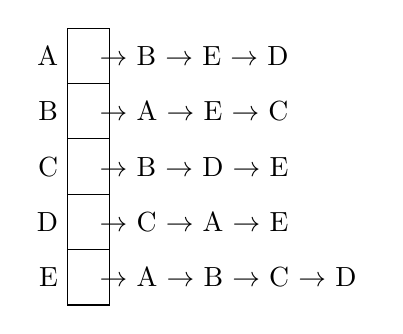
\begin{tikzpicture}
\coordinate (0);
\foreach \foo/\t[count=\i from 0,evaluate=\i as\j using int(\i+1)] in {
  A/B  $\rightarrow$ E $\rightarrow$ D,
  B/A  $\rightarrow$ E $\rightarrow$ C,
  C/B  $\rightarrow$ D $\rightarrow$ E,
  D/C  $\rightarrow$ A $\rightarrow$ E,
  E/A  $\rightarrow$ B $\rightarrow$ C $\rightarrow$ D 
}
\node at(\i.south)[anchor=north,draw,minimum height=2em,minimum width=1.5em,outer sep=0pt](\j){}
    node at(\j.west)[align=right,left]{\foo} 
    node at(\j.east)[align=left,right,xshift=-.7em]{$\rightarrow$ \t};
\end{tikzpicture}
\end{document}